% !TeX spellcheck = en_GB
\section{System Thinking and System Dynamics}

\subsection{Basic Concepts}

\subsubsection{Linear Thinking}
In linear thinking there are no feedbacks possible. Every connection
has a influence on one single variable. The different variables have no
connection whatsoever.

\begin{figure}[H]
	\centering
	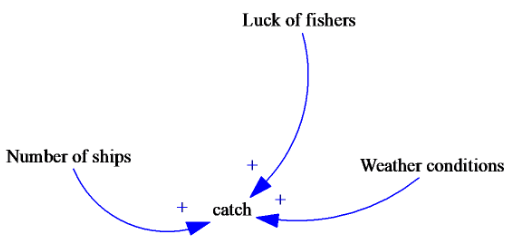
\includegraphics[width=.4\textwidth]{figures/linearThinking.png}
	\caption{CLD of linear thinking}
\end{figure}

\subsubsection{Feedback Thinking}

We derive the essential dynamics from the mechanisms within the system
boundaries.

\begin{figure}[H]
	\centering
	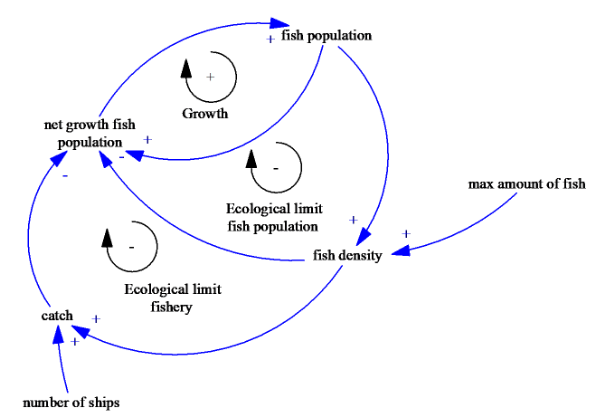
\includegraphics[width=.4\textwidth]{figures/feedbackThinking.png}
	\caption{CLD of feedback thinking}
\end{figure}

With feedback the catch will decrease due to multiple boats because the
sea is getting out fished (but I have no idea, I'm from Switzerland). In
linear think such a behaviour would not be possible.

\subsubsection{Goals}

\begin{description}
	\item[Understanding, not forecasting]
	The goal of a system dynamics policy study is understanding the
	interactions in a complex system that are conspiring to create a
	problem, and understanding the structure and dynamic implications of
	policy changes intended to improve the system's behaviour.
	\item[Modeling for learning]
	Therefore, the primary goal is not to build the model of the system, but
	rather to get a group engaged in building a system dynamics model of a
	problem in order to see to what extent this process might be helpful to
	increase problem understanding and to devise courses of action to which
	team members feel committed.
\end{description}

\subsubsection{Visualization/Representation formats}

\begin{enumerate}
	\item Casual Loop Diagrams (''Communication-tool for a shared mental model
	and general discussion'')
	\item Stock and flow diagrams
	\item Stock and flow diagrams with equations (formulation of all flows as
	equations. This enables quantitative simulation)
\end{enumerate}

\subsection{Causal Loop Diagram (CLD)}

A causal loop diagram (CLD) is a causal diagram that aids in visualizing how
different variables in a system are interrelated. The diagram consists of a set
of nodes and edges. Nodes represent the variables and edges are the links that
represent a connection or a relation between the two variables.

\subsubsection{Link types and loops}

\begin{description}
	\item[Positive polarity] Increases (decreases) cause, then increases
	(decreases) effect.
	\item[Negative polarity] Increases (decreases) cause, then decreases
	(increases) effect.
	\item[Reinforcing Loop] The reinforcement increases the initial effect.\\
	\textbf{A loop is reinforced when the number of minuses is even.}
	\item[Balancing Loop] The feedback balances the initial effect.\\
	\textbf{A loop is balanced if the number of minuses are odd.}
\end{description}

\begin{figure}[H]
\centering
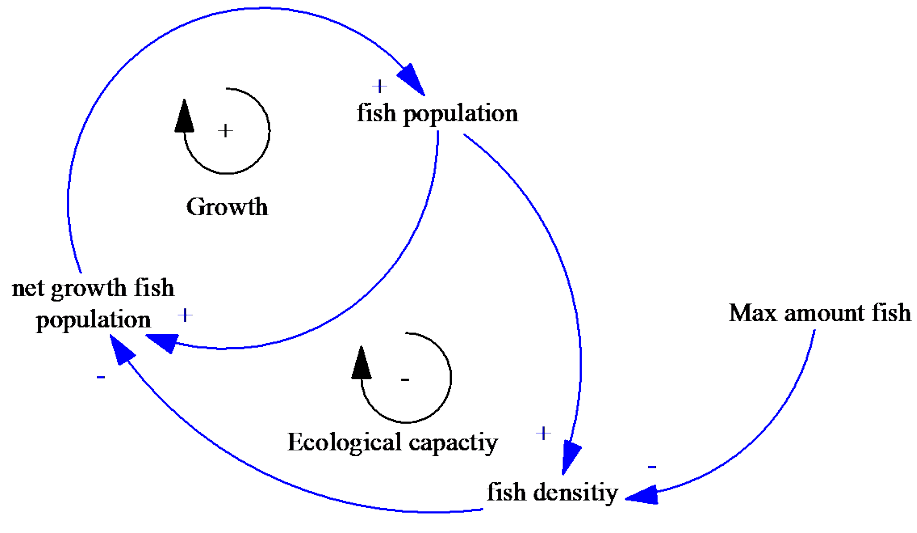
\includegraphics[width=.6\textwidth]{figures/cldFishpopulation.png}
\caption{Example CLD with reinforced and balanced loop}
\end{figure}

\subsubsection{Benefits}

\begin{itemize}
	\tightlist
	\item Create an overview and understand a complex system
	\item Uncover leverage points
	\item Reduce the complexitiy in finding potential side-effects and feedback
	from policy interventions
	\item Identify dependent variables \& potentially conflicting goals
	\item Improve quality of discussion by precise presentation of the subject
	of matter.
\end{itemize}

\subsubsection{Rules for good CLDs}

\begin{itemize}
	\tightlist
	\item \textbf{Variable name}
	\begin{enumerate}
		\item Select substantives as variable name
		\item Don't indicate the direction of variables via the name
		\item The value of the variable needs to be able to increase or decrease
		– the name ideally describes a continuum
	\end{enumerate}
	\item \textbf{Causal relations}
	\begin{enumerate}
		\item Model causality not correlation
		\begin{itemize}
			\item Include only causality that convinces you.
			\item Finding relevant causal explanations is a creative mission and
			requires an exchange of information of relevant stakeholders.
		\end{itemize}
		\item Modelling causal relations with clear polarity; If no polarity
		can be indicated, the underyling structure needs extended analysis.
		\item No ''Shopping List'' (Rule of thumb: max. 3 Causes for 1 effect)
		\item Avoid redundancy
		\item Ask yourself with every decision rule: Are there unintended
		consequences?
		\item Mark the important delays with //
	\end{enumerate}
	\item \textbf{Loops}
	\begin{enumerate}
		\item Close all loops
		\item Validate ALL Feedback: Which story does the loop tell? Use
		mathematical polarity to validate the loop within your story.
	\end{enumerate}
	\item \textbf{Model}
	\begin{enumerate}
		\item Focus on the purpose
		\begin{itemize}
			\item Which goal variable need to be modelled?
			\item Which stories are important to you and the target group?
		\end{itemize}
	\end{enumerate}
\end{itemize}

\subsection{Accumulation}

\emph{Understanding accumulation is fundamental to understanding system
	behaviour.}

\begin{figure}[H]
	\centering
	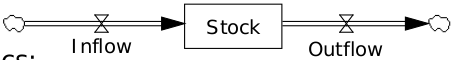
\includegraphics[width=.5\textwidth]{figures/stocknflow.png}
	\caption{Stock and flow diagram}
\end{figure}

\begin{description}
	\item[Stocks] ''Memory'' of a system
	\begin{itemize}
		\tightlist
		\item Need an initial value
		\item Only change via in- and outflows
		\item Have units such as liter, CHF, meter
	\end{itemize}
	\item[Flows] Changing rates of stocks
	\begin{itemize}
		\tightlist
		\item Have units such as liter/h, CHF/year, meter/s
	\end{itemize}
\end{description}

With the stock-and-Flow-Diagram, you show the inflow, the outflow and
the current stock.


\paragraph{Integral equation}
\begin{equation}
Stock(t) = \int_{t_0}^{t}[Inflow(s)-Outflow(s)]ds + Stock(t_0)
\end{equation}

\paragraph{Differential equation}
\begin{equation}
\frac{d}{dt}Stock(t)=Inflow(t)-Outflow(t)
\end{equation}

\emph{A stock takes time to change, because flows take time to flow.
	That's a vital point, a key to understanding why systems behave as they
	do.}

\subsubsection{Difference Between Casual Loop Diagram and Stock-and-Flow Diagram}

\begin{figure}[H]
	\centering
	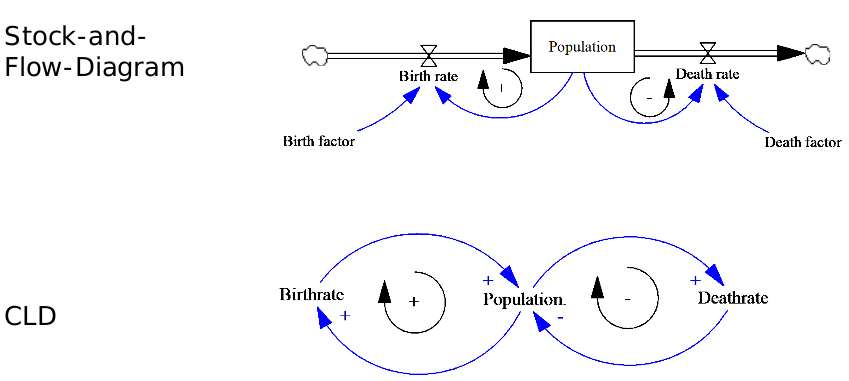
\includegraphics[width=.6\textwidth]{figures/cldVsStockFlow.png}
	\caption{Comparison of a CLD and Stock and Flow diagram}
\end{figure}

\subsection{Limits of casual loop diagrams}

\begin{figure}[H]
	\centering
	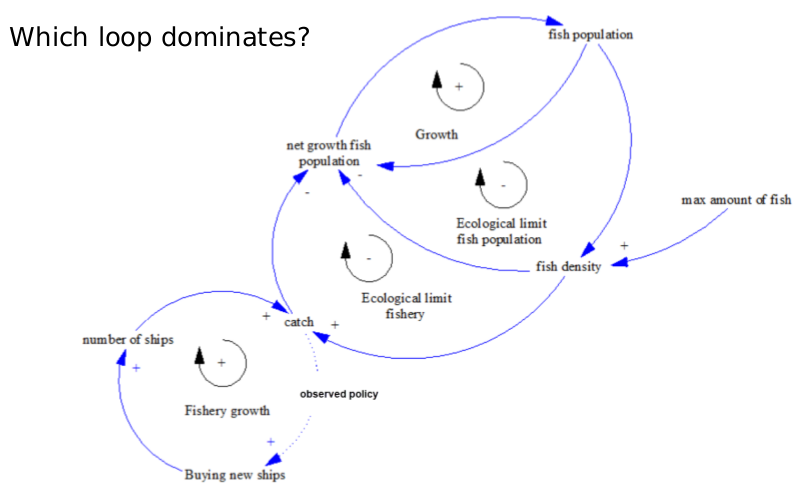
\includegraphics[width=0.7\textwidth]{figures/limitsCld.png}
	\caption{Limits of CLDs}
\end{figure}

\begin{description}
	\item[Domination] With CLDs only and no simulation model, it is not possible
	to determine which loop dominates.
	\item[Collapse point of a system] Saturation points are not modelled. Like
	when are enough fish in the	sea.
	\item[Loop interaction] On basis of the CLD it is not possible to figure
	out, how the loops will interact. The importance of the loops are not
	modelled.
\end{description}

\subsection{Fundamental modes of dynamic behaviour}

This chapter describes common models of dynamic behaviour and shows their
representing CLD.

\subsubsection{Exponential growth}

\begin{figure}[H]
	\centering
	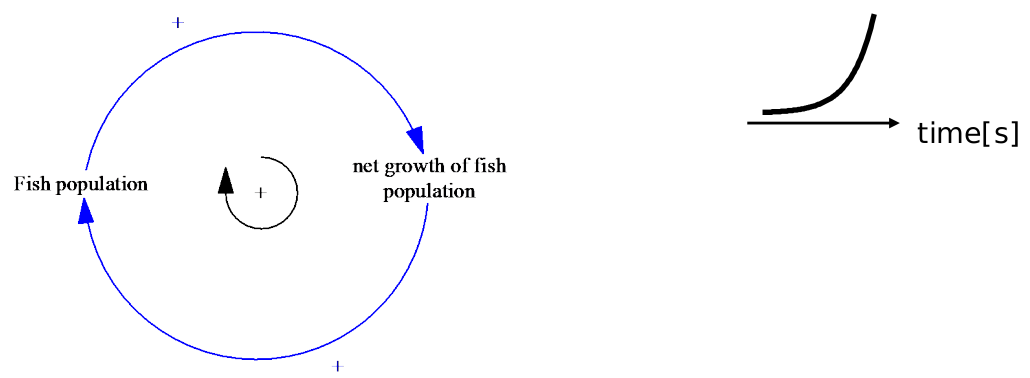
\includegraphics[width=0.6\textwidth]{figures/ExponentialGrowthCLD.png}
	\caption{CLD of an exponential growth}
\end{figure}


\subsubsection{Goal seeking}
\begin{figure}[H]
	\centering
	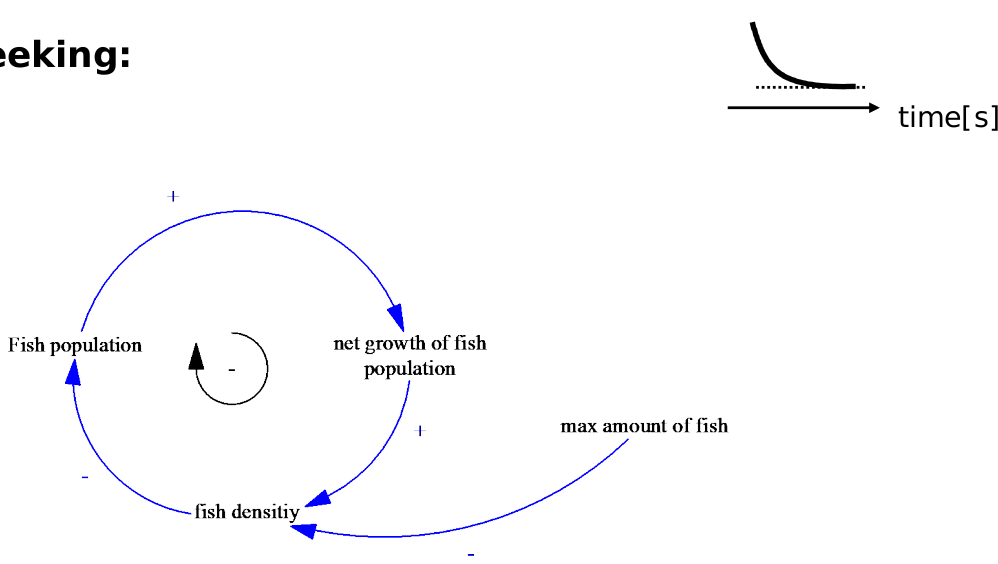
\includegraphics[width=0.6\textwidth]{figures/GoalSeekingCLD.png}
	\caption{CLD of a goal seeking behaviour}
\end{figure}

\subsubsection{Oscillation}
\begin{figure}[H]
	\centering
	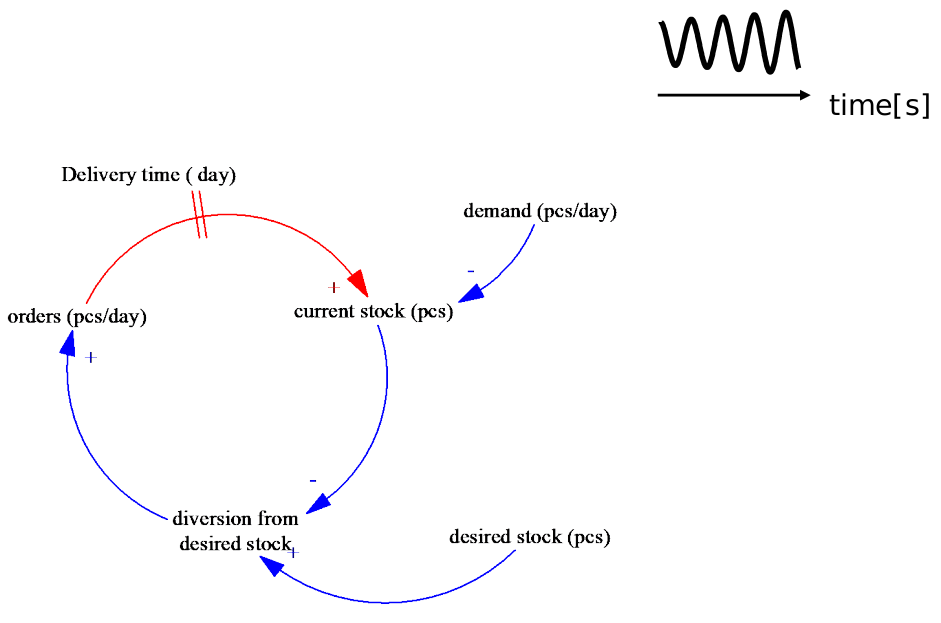
\includegraphics[width=0.6\textwidth]{figures/OscillationCLD.png}
	\caption{CLD which causes a oscillation}
\end{figure}

\subsubsection{S-shaped}
\begin{figure}[H]
	\centering
	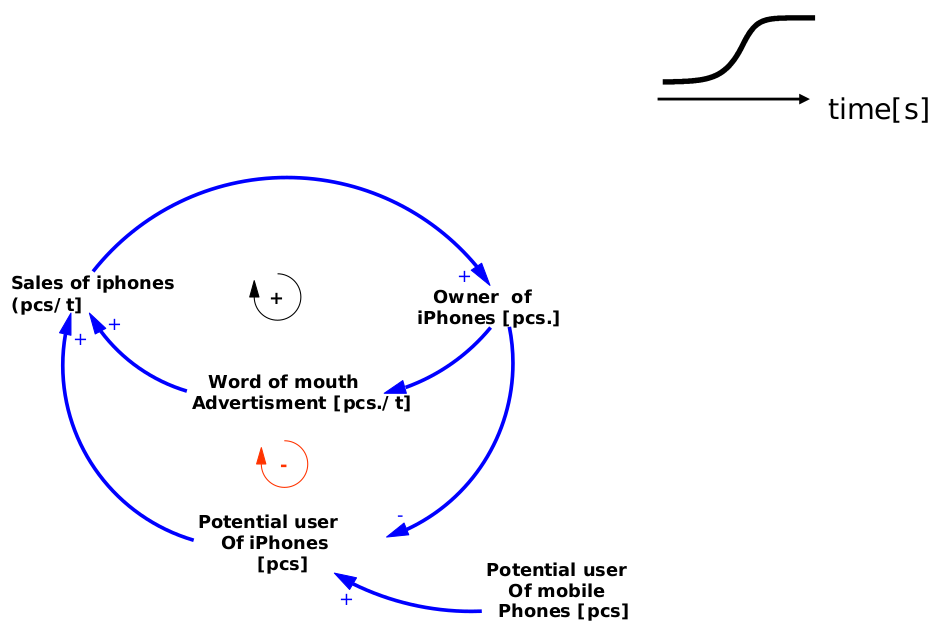
\includegraphics[width=0.6\textwidth]{figures/SShapedCLD.png}
	\caption{CLD which results in an S-shaped behaviour}
\end{figure}

\subsubsection{Growth and overshoot}
\begin{figure}[H]
	\centering
	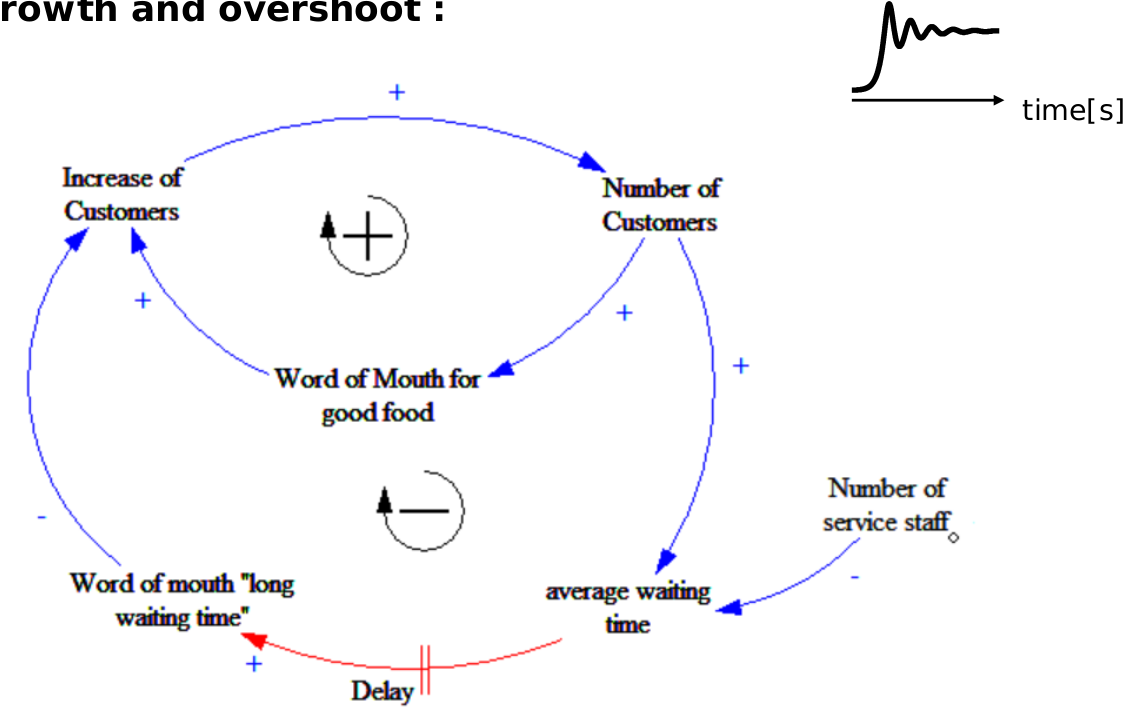
\includegraphics[width=0.6\textwidth]{figures/GrowthOvershootCLD.png}
	\caption{CLD grows and overshoots}
\end{figure}

\subsubsection{Overshoot and collapse}
\begin{figure}[H]
	\centering
	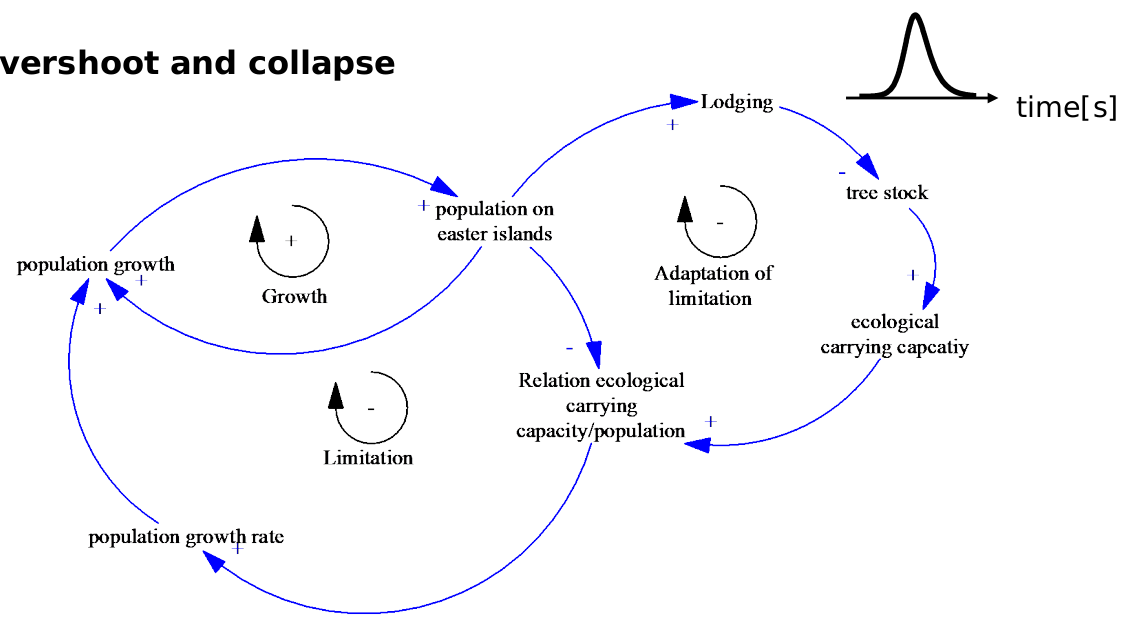
\includegraphics[width=0.6\textwidth]{figures/OvershootCollapseCLD.png}
	\caption{CLD overshoots and then collapses}
\end{figure}

\subsection{Path Dependency}

A \textbf{Lock-in-situation} occurs \textit{based upon decisions in the past},
\textit{when changing the current situation is linked to high investment} and
\textit{therefore doesn't happen often.}

\paragraph{Examples}

\begin{itemize}
	\item QWERTY-Keyboard
	\item Fossil fuel powered civilization
	\item Gender roles
\end{itemize}

\subsubsection{Polya-Process}

The Polya-Process is a well known experiment to demonstrate a \textbf{Lock-in
situation}.

\begin{figure}[H]
	\centering
	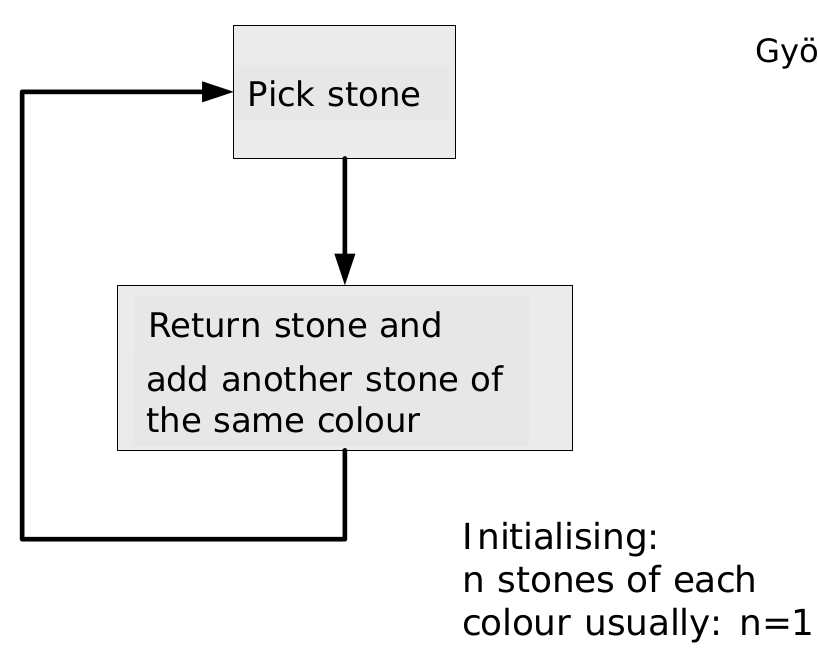
\includegraphics[width=0.4\textwidth]{figures/PolyaProcess.png}
	\caption{Flowchart of the Polya-Process}
\end{figure}

\begin{figure}[H]
	\centering
	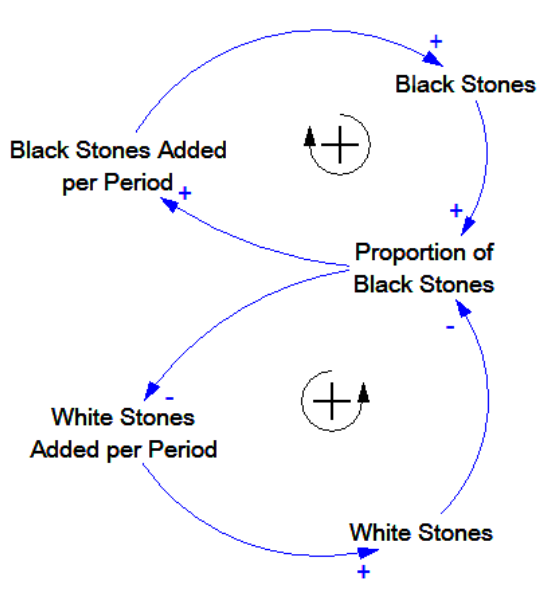
\includegraphics[width=0.4\textwidth]{figures/PolyaProcessCLD.png}
	\caption{CLD of the Polya-Process}
\end{figure}
